\section{应用随机过程部分}
\begin{center}
    Instructor: Pengkun Yang 
\end{center}

% \subsection{Review of Probability}
    





\subsection{Minimum Mean Squared Estimator}\label{SubSecMMSE}
    Motivation: Here's a signal transmission process in which source is $ X\sim f_{X} $ and observation is $ \vec{Z}\sim f_Z $, we need to find a (theoretically best) information process function $ g(\, \cdot \, ) $ such that we can reproduce $ X $ with $ g(\vec{Z}) $ with minimum `error' (Note that $ X$ and $\vec{Z} $ can be dependent)., i.e.
    \begin{align}
        \hat{g}=\mathop{\arg\min}\limits_{g(\, \cdot \, )\in \mathscr{F}} \mathbb{E}\left[ (X-g(\vec{Z}))^2 \right] 
    \end{align}

    which is the \textbf{Minimum Mean Squared Estimator} (MMSE)\index{MMSE (Minimum Mean Squared Estimator)}. \footnote{\textbf{Note}: the function space $ \mathscr{F}(\vec{Z}) $ (by default) is the arbitrary measurable function space $ :=\mathscr{V}(\vec{Z}) $, but you can specifically select a proper one, e.g. linear combination of some power function $ \mathbb{V}(1,\vec{Z},\vec{Z}^2):=\{a+bZ+cZ^2\}_{a,b,c\in\mathbb{R}}\subset \mathscr{F}(\vec{Z}) $.
    
    I am not quite sure (actually I believe it's wrong lol) but maybe for some commonly used function form, we could view that
    \begin{align}
        \mathscr{V}(\vec{Z})\approx \mathbb{V}(\{\vec{Z}^p\}_{p=-\infty}^\infty) 
    \end{align}
    
    }

\begin{point}
    General Solution to MMSE
\end{point}

    The solution to MMSE is that
    \begin{align}
         \hat{g}(\, \cdot \, )\, s.t. \begin{cases}
            \hat{g}(\vec{Z})\in \mathscr{F}(Z)\\
            e:=X-\hat{g}(\vec{Z})\perp h(\vec{Z}),\quad \forall h(\vec{Z})\in\mathscr{F}(Z)
         \end{cases}
    \end{align}
    
    here $ \perp $ in the sense that $ \imath \perp \jmath \Leftrightarrow \mathbb{E}\left[ \imath\jmath \right]=0  $
    
    \begin{proof}
        Denote $ \mathscr{F}(Z)\ni g(Z)=\hat{g}(Z)+c h(Z)  ,\,h(Z)\in\mathscr{F}(Z)$, then
        \begin{align}
            \mathbb{E}\left[ (X-g(Z))^2 \right]  =&\mathbb{E}\left[ (X-\hat{g}(Z)-ch(Z))^2 \right]\\
            =&\mathbb{E}\left[ (X-\hat{g}(Z))^2 \right] -2c\mathbb{E}\left[ (X-\hat{g}(Z))h(Z) \right]+c^2\mathbb{E}\left[ h(Z)^2 \right]  
        \end{align}
        
        \begin{itemize}[topsep=2pt,itemsep=0pt]
            \item If $ X-\hat{g}(\vec{Z})\perp h(\vec{Z})  $: $
                \mathbb{E}\left[ (X-g(Z))^2 \right]  =\mathbb{E}\left[ (X-\hat{g}(Z))^2 \right] +c^2\mathbb{E}\left[ h(Z)^2 \right]  \geq \mathbb{E}\left[ (X-\hat{g}(Z))^2 \right]$
            \item If $ X-\hat{g}(\vec{Z})\not\perp h(\vec{Z})  $, then for $ |c| $ small enough we could have $ \mathbb{E}\left[ (X-g(Z))^2 \right]< \mathbb{E}\left[ (X-\hat{g}(Z))^2 \right]$.          
        \end{itemize}
        
        which gives that the above condition is  necessary and sufficient.
    \end{proof}
    
    
    
    The above expression is similar to the projection operator onto space $ \mathscr{F} $, i.e.
    \begin{align}
        \hat{g}(\, \cdot \, )=\Pi_{\mathscr{F(\, \cdot \, )}}(X),\quad \begin{cases}
            \Pi_{\mathscr{F(\, \cdot \, )}}(X)\in \mathscr{F}\\
            X-\Pi_{\mathscr{F(\, \cdot \, )}}(X)\perp \mathscr{F}
        \end{cases}
    \end{align}
    
\begin{point}
    Properties of Projection Operator $ \Pi_{\mathcal{V}} $ (where function space $ \mathscr{F} $ is a kind of linear space $ \mathcal{V} $)\index{Projection Operator}
\end{point}
\begin{itemize}[topsep=2pt,itemsep=0pt]
    \item Linearity
    \begin{align}
        \Pi_{\mathcal{V}}(aX+bY)=a\Pi_{\mathcal{V}}(X)+b\Pi_{\mathcal{V}}(Y)
    \end{align}
    \item Project within subspace: for $\mathcal{V}_2\subset \mathcal{V}_1 $
    \begin{align}
        \Pi_{\mathcal{V}_2}(X)=\Pi_{\mathcal{V}_2}\left(\Pi_{\mathcal{V}_1}(X)\right) 
    \end{align}
    \item Projection onto orthogonal space: for $ \mathcal{V}_1\perp\mathcal{V}_2 $
    \begin{align}
        \Pi_{\mathcal{V}_1\oplus\mathcal{V}_2}(X)=\Pi_{\mathcal{V}_1}(X)+\Pi_{\mathcal{V}_2}(X) 
    \end{align}
\end{itemize}

\begin{point}
    Important Cases
\end{point}

\begin{itemize}[topsep=2pt,itemsep=0pt]
    \item $ \mathscr{F}(Z)=\mathscr{V}(Z) $: Solution is 
    \begin{align}
        \mathbb{E}\left[ X|Z \right] 
    \end{align}
    
    in which
    \begin{align}
        \begin{cases}
            \mathbb{E}\left[ X|Z \right] \in\mathscr{F}(Z)\\
            \mathbb{E}\left[(X-\mathbb{E}\left[ X|Z \right] )g(Z) \right]=\mathbb{E}\left[ Xg(Z) \right] -\mathbb{E}\left[ \mathbb{E}\left[ g(Z)X|Z \right]  \right] =0 
        \end{cases} 
    \end{align}
    \item $ \mathscr{F}(Z)=\mathrm{const} $: Solution is
    \begin{align}
         \mathbb{E}\left[ X \right]  
    \end{align}
    
    in which
    \begin{align}
        \begin{cases}
            \mathbb{E}\left[ X \right]\in \mathcal{R}\\
            \mathbb{E}\left[ (X-\mathbb{E}\left[ X \right] )\mathrm{const} \right]=0 
        \end{cases} 
    \end{align}

    which is also a kind of variance definition:
    \begin{align}
        var(X):=\min_{c\in\mathbb{R}}\mathbb{E}\left[ (X-c)^2 \right]  
    \end{align}
    
    \item \hypertarget{MMSELinear}{}$ \mathscr{F}(Z)=\mathbb{V}(1,\vec{Z}) $ i.e. linear conbination of $ \vec{Z} $ as $ a+\vec{Z}'b $. Solution is
    \begin{align}
        L(X|\vec{Z}):=\mathbb{E}\left[ X \right] +cov(X,\vec{Z})var(\vec{Z})^{-1}\left(\vec{Z}-\mathbb{E}\left[ \vec{Z} \right] \right)
    \end{align}
    
    in which
    \begin{align}
        \begin{cases}
            \mathbb{E}\left[ X \right] +cov(X,\vec{Z})var(\vec{Z})^{-1}\left(\vec{Z}-\mathbb{E}\left[ \vec{Z} \right] \right)\in \mathbb{V}(1,\vec{Z})\\
        \mathbb{E}\left[ (X-L(X|\vec{Z}))(a+\vec{Z}'b) \right] = 0
        \end{cases}
    \end{align}
    
\end{itemize}


\begin{point}
    Innovation Sequence (新息序列)\index{Innovation Sequence}
\end{point}

Motivation: construction of linear MMSE $ L(X|Y_1,Y_2,\ldots,Y_n)=L(X|Y) $. Assume that $\mathbb{E}\left[ \vec{Y} \right] =0 $, the prediction is
\begin{align}
    L(X|\vec{Y})=\mathbb{E}\left[ X \right] + cov(X,\vec{Y})var(\vec{Y})^{-1}\vec{Y}
\end{align}
which causes the problem of computation complexity when $ n $ is large. 

Innovation sequence fixed this problem by: instead of projecting on the whole linear combination $ \vec{Y} $ space of size $ (n+1) $, we project on space of each $ Y_i $ sequentially. i.e. define an \textbf{innovation sequence} 
\begin{align}
    \tilde{Y}_1=&Y_1\\
    \tilde{Y}_2=&Y_2-L(Y_2|Y_1)\\
    \tilde{Y}_3=&Y_3-L(Y_3|Y_2Y_1)\\
    \ldots&\\
    \tilde{Y}_n=&Y_n-L(Y_n|Y_{n-1}\ldots Y_2Y_1)
\end{align}
where `innovation' means each $ \tilde{Y}_i $ contains the `new information without correlation with previous sequence' $ \mathbb{E}\left[ \tilde{Y_i}\tilde{Y}_j \right]=0\,\forall i\neq j  $. In this way the linear MMSE could be written as
\begin{align}
    L(X|\vec{Y})=L(X|\vec{\tilde{Y}})= \mathbb{E}\left[ X \right] +\sum_{i=1}^n \dfrac{cov(X,\tilde{Y}_i)}{var(\tilde{Y}_i)}\tilde{Y}_i
\end{align}

I think the idea here is similar to Gram-Schmidt orthogonalization (\autoref{SubSubSectionQRDecomposition}), in which we also construct new components by eliminating projection on previous parts. As a result we have a set of orthogonal elements (here orthogonal means $ \mathbb{E}\left[ \tilde{Y}_i\tilde{Y}_j \right]=0  $ and in Gram-Schmidt means $ q_i'q_j = 0 $, $ i\neq j $).






\subsection{Markov Process}
% (Or sometimes called random process)

\subsubsection{Basic Concepts}
Some basic concepts about stochastic process / random process are introduced in \autoref{SubSectionStochasticProcessForTimeSeries}. Here's a brief recap.

A stochastic process is a mapping
\begin{align}
     \{X_t:t\in\mathcal{T}\}:\, \mathcal{T}\times\Omega \mapsto \mathbb{R}
\end{align}

\begin{itemize}[topsep=2pt,itemsep=0pt]
    \item For each given $ t \in\mathcal{T}$, $ X_t(\, \cdot \, ) $ is a r.v. defined on $ \Omega  $.
    \item For each given $ \omega \in \Omega  $, $ X_\cdot (\omega ) $ is a function on $ \mathcal{T} $, which is called sample path.\index{Sample Path}
\end{itemize}

According to the continuity of index set $ \mathcal{T} $ and sample path values, Stochastic process can be categorized in discrete / continuous Time + discrete / continuous State processes.

Some functions of stochastic processes include
\begin{itemize}[topsep=2pt,itemsep=0pt]
    \item Mean function:
    \begin{align}
        \mu _X(t)=\mathbb{E}\left[ X_t \right]  
    \end{align}
    \item AutoCovariance function (ACVF):
    \begin{align}
        \gamma _{s,t}:=cov(X_s,X_t)
    \end{align}
    \item AutoCorrelation function (ACF):
    \begin{align}
        \rho _{s,t}:=corr(X_s,X_t)=\dfrac{\gamma _{s,t}}{\sqrt{\gamma _{s,s}\gamma _{t,t}}} 
    \end{align}
    \item $ n^\mathrm{th}  $ order CDF:
    \begin{align}
        F_{X,n}(x_1,t_1;x_2,t_2;\ldots;x_n,t_n)=\mathbb{P}\left( X_{t_1}\leq x_1,\,X_{t_2}\leq x_2,\ldots,\,X_{t_n}\leq x_n \right)  
    \end{align}
   
\end{itemize}

% \begin{point}
%     Some Examples 
% \end{point}

% \begin{itemize}[topsep=2pt,itemsep=0pt]
%     \item Trajectory of horizontal projectile motion with random initial height $ A\sim f_A $ and initial velocity $ B\sim f_B $:
%     \begin{align}
%         Y_t=-\dfrac{1}{2}gt^2+B(\omega _B)t+A(\omega _A)
%     \end{align}

%     with 
%     \begin{align}
%         \gamma _{s,t}=1+st,\quad \rho _{s,t}=\dfrac{1+st}{\sqrt{(1+s^2)(1+t^2)}}  
%     \end{align}
    
    
%     \item 
    
    
% \end{itemize}

    


\subsubsection{Conditional Independence}
Conditional independence \index{Conditional Independence}: say $ X $ and $ Z $ are conditionally independent given $ Y $, i.e. $ X $-$ Y $-$ Z $
\begin{align}
    f_{X|YZ}=f_{X|Y}\Leftrightarrow f_{XZ|Y}=f_{X|Y}f_{Z|Y} 
\end{align}

Further if $ (X,Y,Z)\sim N(\mu ,\Sigma ) $ (a joint Gaussian Dist.). Then
\begin{align}
    cov(X,Z)=cov(X,Y)var(Y)^{-1}cov(Y,Z)
\end{align}
it could be deduced using linar MMSE + innovation sequence of jointly Gaussian
\begin{align}
    cov(Z,X-L(X|Y))=0\Rightarrow cov(X,Z)= cov(X,Y)var(Y)^{-1}cov(Y,Z)
\end{align}
or use \autoref{EquConditionalPrForGaussian}, in which $ X_1=(X,Z),\,X_2=Y $
\begin{align}
    \Sigma _{X,Z|Y}=\begin{bmatrix}
        \Sigma _{X}-\Sigma _{XY}-\Sigma _{Y}^{-1}\Sigma _{YX}&\Sigma _{XZ}-\Sigma _{XY}\Sigma _{Y}^{-1}\Sigma _{YZ}\\
        \Sigma _{ZX}-\Sigma _{ZY}\Sigma _Y^{-1}\Sigma _{YX}&\Sigma _{Z}-\Sigma _{ZY}\Sigma _Y^{-1}\Sigma _{YZ}
    \end{bmatrix} \Rightarrow \Sigma _{XZ}-\Sigma _{XY}\Sigma _{Y}^{-1}\Sigma _{YZ}=0
\end{align}





\subsubsection{Properties of Discrete Time Markov Chain}\label{SubSubSectionDTMC}
A basic case for Markov Chain is Discrete Time Markov Chain (DTMC)\index{DTMC (Discrete Time Markov Chain)}

\begin{point}
    Notations and Properties of DTMC
\end{point}
\begin{itemize}[topsep=2pt,itemsep=0pt]
    \item State: denote the state space / phase space of DTMC as
    \begin{align}
        X_n\in \mathcal{S} 
    \end{align}
    \item Conditional Independency: 
    \begin{align*}
         \mathbb{P}\left( X_{n+1}\big|X_0,X_1,\ldots,X_n \right)=\mathbb{P}\left( X_{n+1}\big|X_n \right)  
    \end{align*}
    
    
    \item State transition and transition probability matrix:
    \begin{align}
        P^{(k)}=\left\{P^{(k)}_{ij}\right\}=\left\{ \mathbb{P}\left( X_{k+1}=j\big| X_{k}=i \right)  \right\},\quad i,j\in \mathcal{S}
    \end{align}
    transition pr matrix $ P $ is called a (row) stochastic matrix, with
    \begin{align}
        0\leq P^{(k)}_{ij}\leq 1,\quad \sum_{j}P^{(k)}_{ij}=1 
    \end{align}

    \item Time homogeneity: transition probability is independent of step / time
    \begin{align}
        P^{(k)}=P,\quad \forall k 
    \end{align}
    we usually focus on time-homogeneous DTMC.
    
    \item State diagram: a useful way to visualize DTMC, in which vertices / nodes for states and edges / arrows for transition. Here's an example of `Mickey Mouse' diagram with six states:
    \begin{center}
        $
            P=\begin{pNiceMatrix}[first-row,first-col]
                &0&1&2&3&4&5\\
                0&&4/9&&&&5/9\\
                1&1/9&4/9&4/9&&&\\
                2&&4/9&4/9&1/9&&\\
                3&&&4/9&&5/9&\\
                4&&&&&&1\\
                5&&&&&&1
            \end{pNiceMatrix}\qquad \quad\bm{\leftrightharpoons }
        $
        \begin{tikzpicture}[baseline={([yshift = -5ex]current bounding box.center)}]
            \GraphInit[vstyle=Dijkstra]
            \SetGraphUnit{2}
            
            \Vertices[Lpos=45]{circle}{0,1,2,3,4,5}

            \tikzset{LabelStyle/.style={fill = white},
            EdgeStyle/.style={-stealth}}
            \Loop[dist = 2cm, dir = NOEA, label = 4/9](1)
            \Loop[dist = 2cm, dir = NOWE, label = 4/9](2)

            \tikzset{EdgeStyle/.style={-stealth, bend right}}
            \Edge[label = 4/9](0)(1)
            \Edge[label = 1/9](1)(0)
            \Edge[label = 4/9](1)(2)
            \Edge[label = 4/9](2)(1)
            \Edge[label = 1/9](2)(3)
            \Edge[label = 4/9](3)(2)
            \Edge[label = 5/9](3)(4)
            \Edge[label = 1](4)(5)

            \tikzset{EdgeStyle/.style={-stealth, bend left}}
            \Edge[label = 5/9 ](0)(5)
          \end{tikzpicture}
        \end{center}
\end{itemize}

\begin{point}
    Stationary Distribution
\end{point}

    State transition between steps are like jumping in state diagram. Denote $ \pi(k) $ the probability distribution at step $ k $, then a transition is
        \begin{align}
            \pi({k+1})=\pi(k)P^{(k)}=\pi(k)P 
        \end{align}

        A stationary distribution / equilibrium of DTMC is the eigen distribution of transition matrix
        \begin{align}
            \pi^*=\pi^*P=\pi^*P^i,\,\forall i 
        \end{align}
        
        A sufficient condition for stationary state is the detailed balance condition\index{Detailed Balance Condition}
        \begin{align}
            &\pi^*_i=\sum_{j}\pi^*_jP_{ji}\\
            \Leftrightarrow&\pi^*\sum_{j\neq i}P_{ij}=\pi^*_i(1-P_{ii})=\sum_{j\neq i}\pi^*jP_{ji}\\
            \Leftarrow&\color{red}\pi_iP_{ij}=\pi_jP_{ji}
        \end{align}

        Some concepts related to stationary distribution
    \begin{itemize}[topsep=2pt,itemsep=0pt]
        \item Reachable: we can arrive at $ j $ starting from $ i $, denoted $ i\leadsto j $
        \begin{align}
            \exists n<\infty s.t. \mathbb{P}\left( X_n=j|X_0=i \right) > 0 
        \end{align}

        Sometimes I use the notation $ i\xrightarrow[]{k}j  $ for `reaching $ j $ in $ k $ steps from $ i $'
        \item Irreducible\index{Irreducible}: every state is reachable from any other states
        \begin{align}
            i\leadsto j,\,\forall i,j\in\mathcal{S} 
        \end{align}
        
        \item Periodic: the period $ d_i $ for state $ i $ is the greatest common divisor (GCD)\index{GCD (Greatest Common Divisor)} of step-to-come-back.
        \begin{align}
            d_i:=\gcd\left\{ n:\mathbb{P}\left( X_n=i|X_0=i \right)>0  \right\} 
        \end{align}

        Irreducible DTMC has the same period for all states.

        \begin{proof}
            For any two states $ i $, $ j $, with periods $ d_i $, $ d_j $. Then $ d_i $ contains the following process:
            \begin{align}
                \{i\xrightarrow[]{k_1}j\xrightarrow[]{m\times d_j}j\xrightarrow[]{k_n}i \} ,\quad m\in\mathbb{N}
            \end{align}
            there are infinite elements. then
            \begin{align}
                d_i=\mathrm{cd} \left\{ k_1+k_2+md_j;m=0,1,2,\ldots \right\} \Rightarrow d_j=\text{multiple of }d_i
            \end{align}
         
            With the argument applied to all state pairs $ (i,j)\in\mathcal{S}\times \mathcal{S} $, obviously $ d_i=d,\,\forall i\in\mathcal{S} $
        \end{proof}
        \item Aperiodic\index{Aperiodic}: is the case that $ d_i=1 $, i.e. possible to come back anytime. For irreducible DTMC, if one state is aperiodic, then all are.        
        
        Naturally if a node is self looped $ P_{ii}>0 $ (e.g. node 1 or 2 in `Mickey Mouse' loops back with pr $ 4/9 $), then all the states are aperiodic.
        \item Sojourn Time\index{Sojourn Time} $ T_i $: is the time to stay at the state
        \begin{align}\label{EqaDTMCSojournTime}
            T_i\sim \mathrm{Geo}(1-P_{ii})  
        \end{align}
        \item Classification of States. 
        
        Denote Hitting Time (without itself include) $ \tau_i^+ $ and its mean 
        \begin{align}
            \tau_i^+:=&\min\{k\geq 1:X_k=i\}\\
            \mu _i:=&\mathbb{E}\left[ \tau_i^+|X_0=i \right] 
        \end{align}
        
        \begin{itemize}[topsep=2pt,itemsep=0pt]
            \item Recurrent State
            \begin{align}
                \mathbb{P}\left( \tau_i^+<\infty|X_0=i    \right)=1  
            \end{align}
            in which 
            \begin{itemize}[topsep=2pt,itemsep=0pt]
                \item Positive Recurrent
                \begin{align}
                    \mu _i<\infty 
                \end{align}
                \item Null Recurrent
                \begin{align}
                    \mu _i=\infty 
                \end{align}

                An example:
                \begin{center}
                \begin{tikzpicture}
                \GraphInit[vstyle=Dijkstra]
                \SetGraphUnit{2}
                    \tikzset{VertexStyle/.style = {
                        shape = rectangle,
                        color = black,
                        text = black,
                        inner sep = 2pt,
                        outer sep = 2pt,
                        draw}}
                    \Vertices{line}{1,2,3,4}
                    \EA[L=$3^k-1$](4){8}
                    \EA[L=$ 3^k $](8){9}
                    \EA[L=$ 3^k+1 $](9){10}
                    \tikzset{VertexStyle/.style = {
                        shape = circle,
                        color = white,
                        text = black,
                        minimum size = 23pt,
                        draw}}
                
                    \EA[L=...,unit=0.8 ](4)(5)
                    \EA[L=...,unit=1.2 ](10)(11)

                    \tikzset{EdgeStyle/.style = {->,bend left,thick}}
                    \tikzset{LabelStyle/.style = {fill=white}}

                    \Edge[label=1/2](3)(1)
                    \Edge[label=1/2](9)(1)

                    \Edge[label=1/2](3)(4)
                    \Edge[label=1/2](9)(10)

                    \Edge[label=1](1)(2)
                    \Edge[label=1](8)(9)
                    \Edge[label=1](2)(3)

                \end{tikzpicture}
                \end{center}

                where 
                \begin{align}
                    \mu _1=\mathbb{E}\left[ \tau_1^+|X_0=1 \right]=\sum_{i=1}^\infty \left(\dfrac{3}{2}\right)^i\to\infty   
                \end{align}
                
                

            \end{itemize} 
            \item Transient State
            \begin{align}
                \mathbb{P}\left( \tau_i^+<\infty|X_0=i    \right)<1 
            \end{align}
        \end{itemize}
        
            
    \end{itemize}
    
\begin{point}
    DTMC: Irreducible \& Aperiodic \& Positive Recurrent $ \Rightarrow  $ Unique Stationary Distribution $ \pi^* $ Exists
\end{point}

Given irreducible \& aperiodic DTMC, we have 

\begin{itemize}[topsep=2pt,itemsep=0pt]
    \item All states have the same state classification: null recurrent / positive recurrent / transient.
    \item if all states are positive recurrent $ \mu _i<\infty $, then stationary distribution exists.
    \begin{align}
        \lim_{n\to \infty}\dfrac{1}{n}\sum_{l=1}^n(P^l)_{ij}=\dfrac{1}{\mu _i}\Rightarrow \pi_i(\infty)=(\pi(0)P^\infty)_i= \dfrac{1}{\mu _i},\, \forall \pi(0)
    \end{align}
    \item Further if states are positive recurrent $ \mu _i<\infty $, then $ \pi^*=\pi(\infty)=[1/\mu _i] $ is the stationary distribution.

    (The proof is a little bit complicated = =)
    
\end{itemize}

Some algorithm about Markov Chain see \autoref{SubSubSectionMCMCAlgorithm}.







\subsubsection{Random Walk}

Random walk is a renewal process $ X_n $ with each step $ W_i $ takes value $ \pm 1 $
\begin{align}
    X_n := X_0 +\sum_{i=1}^nW_i\quad W_i=\begin{cases}
        +1&\mathrm{w.p.}\, p\\
        -1&\mathrm{w.p.}\, q:=1-p  
    \end{cases}
\end{align}
where $ X_0=k $ is the initial position.

\begin{point}
    Simple Random Walk
\end{point}

Simple random walk is the case with no ends, i.e. $ X_n\in \mathbb{Z} $


\begin{itemize}[topsep=2pt,itemsep=0pt]
    \item State Diagram for Simple Random Walk
\begin{center}
    \begin{tikzpicture}
    \GraphInit[vstyle=Dijkstra]
    \SetGraphUnit{2}
        \tikzset{VertexStyle/.style = {
            shape = rectangle,
            color = black,
            text = black,
            inner sep = 2pt,
            outer sep = 2pt,
            draw}}
        \Vertex[L=$ k $]{0}
        \EA[L=$k+1$](0){1}
        \EA[L=$k+2$](1){2}
        \WE[L=$k-1$](0){10}
        \WE[L=$k-2$](10){20}
        \tikzset{VertexStyle/.style = {
            shape = circle,
            color = white,
            text = black,
            minimum size = 23pt,
            draw}}
        \EA[L=...,unit=1.9 ](2){3}
        \WE[L=...,unit=1.9 ](20){30}

        \tikzset{EdgeStyle/.style = {->,bend left,thick}}
        \tikzset{LabelStyle/.style = {fill=white}}

        \Edge[label=$ p $](30)(20)
        \Edge[label=$ p $](20)(10)
        \Edge[label=$ p $](10)(0)
        \Edge[label=$ p $](0)(1)
        \Edge[label=$ p $](1)(2)
        \Edge[label=$ p $](2)(3)

        \Edge[label=$ q $](20)(30)
        \Edge[label=$ q $](10)(20)
        \Edge[label=$ q $](0)(10)
        \Edge[label=$ q $](1)(0)
        \Edge[label=$ q $](2)(1)
        \Edge[label=$ q $](3)(2)


    \end{tikzpicture}
    \end{center}
    \item Parameters
    \begin{align}
        \begin{cases}
            \text{Mean Function}:\mu _n=k+n(2p-1)\\
            \text{Covariance}:\gamma _{m,n}=4pq\min\{m,n\}\\
            \text{CLT}:\dfrac{X_n-k-n(2p-1)}{\sqrt{4npq}}\xrightarrow[]{d} N(0,1)
        \end{cases} 
    \end{align}
    
    
\end{itemize}

\begin{point}
    Gambler's Model
\end{point}

Gambler's model is the case with one/two ends, usually one of the ends is denoted $ 0 $, as Gambler's ruin, and the other denoted $ N $ as Gambler's success.

Reaching $ 0 $ or $ N $ stops the chain, so are called `absorbing state'.\index{Absorbing State}

\begin{itemize}[topsep=2pt,itemsep=0pt]
    \item State Diagram of Gambler's model with two ends
    \begin{center}
        \begin{tikzpicture}
        \GraphInit[vstyle=Dijkstra]
        \SetGraphUnit{2}
            \tikzset{VertexStyle/.style = {
                shape = rectangle,
                color = black,
                text = black,
                inner sep = 2pt,
                outer sep = 2pt,
                draw}}
            \Vertex[L=$ 0 $]{0}
            \EA[L=$1$](0){1}
            \EA[L=$2$](1){2}
            \tikzset{VertexStyle/.style = {
                shape = circle,
                color = white,
                text = black,
                minimum size = 23pt,
                draw}}
            \EA[L=$ \ldots $](2){3}
            \tikzset{VertexStyle/.style = {
                shape = rectangle,
                color = black,
                text = black,
                inner sep = 2pt,
                outer sep = 2pt,
                draw}}
            \EA[L=$ N-2 $](3){4}
            \EA[L=$ N-1 $](4){5}
            \EA[L=$ N $](5){6}

            \tikzset{LabelStyle/.style = {fill=white}}
            \Loop[dist = 1.2cm, dir = EA, label = 1](6)
            \Loop[dist = 1.2cm, dir = WE, label = 1](0)

    
            \tikzset{EdgeStyle/.style = {->,bend left,thick}}
            \tikzset{LabelStyle/.style = {fill=white}}
    
            \Edges[label = $ p $](1,2,3,4,5,6)
            \Edges[label = $ q $](5,4,3,2,1,0)
    
        \end{tikzpicture}
        \end{center}
    \item Gambler's Ruin / Success: Denote Hitting Time (allowing itself included)\index{Hitting Time} $\tau_i=\min\left\{ n\geq 0: X_n=i \right\} $, and  probability of ruin $ r_i $ and probability of success $ s_i $ respectively
    \begin{align}
        r_i:=&\mathbb{P}\left( X_{\tau_0}=0|X_0=i \right)\\
        s_i:=&\mathbb{P}\left( X_{\tau_N}=N|X_0=i \right)
    \end{align}
    with itertion relation
    \begin{align}
        s_i=p\cdot s_{i+1}+q\cdot s_{i-1},\quad s_0=0,\,s_N=1\\
        r_i=q\cdot r_{i+1}+p\cdot r_{i-1},\quad r_0=1,\,r_N=0 
    \end{align}

    we could get\footnote{For the case $ q=p=1/2 $, take the natural limit to get corresponding solution
    \begin{align}
        s_i=&\dfrac{k}{N}\\
        r_i=&1-\dfrac{k}{N}
    \end{align}
    }
    \begin{align}
        s_i=&\dfrac{1-(q/p)^i}{1-(q/p)^N}\\
        r_i=&\dfrac{(q/p)^i-(q/p)^N}{1-(q/p)^N}=1-s_i
    \end{align}
    \item Mean Hitting Time $ T_{i\leadsto \{0,N\}} $ for $ i\leadsto \{0,N\} $: $ T_{i\leadsto \{0,N\}}=\mathbb{E}\left[ \min\{\tau_{0},\tau_{N}\}|X_0=i \right]  $:
    \begin{align}
        T_{i\leadsto \{0,N\}}= p\left(1+T_{i+1\leadsto \{0,N\}}\right) + q\left(1+T_{i-1\leadsto \{0,N\}}\right),\quad T_{N\leadsto \{0,N\}}=T_{0\leadsto \{0,N\}}=0
    \end{align}
    solution
\begin{align}
    T_{i\leadsto\{0,N\}}=\dfrac{\left(1-(q/p)^i\right)(N-i)}{\left(1-(q/p)^N\right)(p-q)} 
\end{align}
    \item One-end case (greedy gambler) is just having $ N\to\infty $
    \begin{align}
        r_i=&\begin{cases}
            1,&p\leq \dfrac{1}{2}\\
            \left(\dfrac{q}{p}\right)^i,&p>\dfrac{1}{2}
        \end{cases} 
    \end{align}
    
    Note: i.e. there is a phase transition at $ p=\dfrac{1}{2} $.

\end{itemize}





% polya: for $ d $-dimensional homogeneous random walk, i.e. $ p=1/4 $ for 2 dim, $ p=1/6 $ for 3 dim ... If $ d=1,2 $, null recurrent, If $ d\geq 3 $, transient.


\subsubsection{Branching Process}
\index{Branching Process}\index{Galton-Watson Tree}
Branching process focuses on the case of population growth / epidemic infection / nuclear fission chain reaction, etc. Each steps the state $ X_n $ denotes the number of individuals, update of state is given as
\begin{align}
    X_{t+1} = \sum_{j=1}^{X_{t}}Z_{t,j},\quad Z_{t,j}\text{ i.i.d. }\sim Z_{t},\quad X_0=1
\end{align}
and we usually assume the simple case of $ Z_t\text{ i.i.d. }\sim Z $.
\begin{itemize}[topsep=2pt,itemsep=0pt]
    \item State Diagram
    \begin{center}
        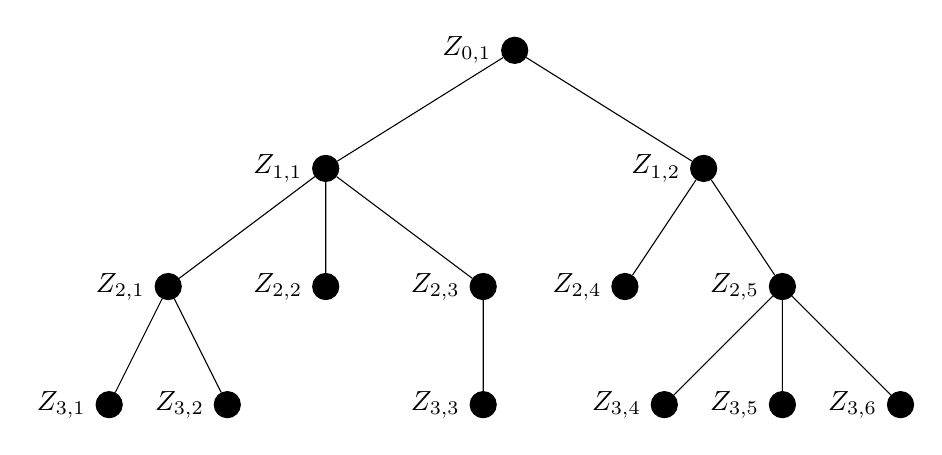
\begin{tikzpicture}[level distance=1.3cm,
        vertex/.style={minimum size=0.5pt,fill,draw,circle},
        level 1/.style={sibling distance=4.8cm, level distance=1.5cm},
        level 2/.style={sibling distance=2cm, level distance=1.5cm},
        level 3/.style={sibling distance=1.5cm, level distance=1.5cm},
        leaf/.style={label={[name=#1]left:$#1$}},
        ]
        \node[vertex, leaf = Z_{0,1}] {}
        child {node[vertex, leaf = Z_{1,1}] {}
            child {node[vertex, leaf = Z_{2,1}] {}
            child {node[vertex, leaf = Z_{3,1}] {}}
            child {node[vertex, leaf = Z_{3,2}] {}}
            }
            child {node[vertex, leaf = Z_{2,2}] {}}
            child {node[vertex, leaf = Z_{2,3}] {}
            child {node[vertex, leaf = Z_{3,3}] {}}
            }
        }
        child {node[vertex, leaf = Z_{1,2}] {}
            child {node[vertex, leaf = Z_{2,4}] {}}
            child {node[vertex, leaf = Z_{2,5}] {}
            child {node[vertex, leaf = Z_{3,4}] {}}
            child {node[vertex, leaf = Z_{3,5}] {}}
            child {node[vertex, leaf = Z_{3,6}] {}}
            }
        };
        \end{tikzpicture}
        \end{center}
    \item $ z $-transform for distribution of $ X_t $:
    \begin{align}
        \Pi_t(s)=\mathbb{E}\left[ s^X_t \right] = \sum_{j=0}^\infty s^j\mathbb{P}\left( X_t=j \right)  \quad L(s)=\mathbb{E}\left[ s^Z \right] =\sum_{j=0}^\infty s^j\mathbb{P}\left( Z=j \right) 
    \end{align}
    and 
    \begin{align}
        \Pi_t(s)=&\sum_{j=0}^\infty \mathbb{E}\left[ s^{X_t}|X_{t-1}=h \right] \mathbb{P}\left( X_{t-1}=j \right) \\
        =&\sum_{j=0}^\infty \left(L(s)\right)^{j}\mathbb{P}\left( X_{t-1}=j \right) \\
        =&\Pi_{t-1}\left(L(s)\right)\\
        (\Pi_1(s)=L(s))=&L^{(t)}(s) 
    \end{align}
    \item Mean and Variance:
    \begin{align}
        \text{Mean}:&\, \mu (t) = \Pi_t'(1)=\mu(0) ^t\\
        \text{Variance}:&\,var(t)=\Pi_t''(1)+\Pi_t'(1)-[\Pi_t'(1)]^2
    \end{align}
    \item Extinction Probability
    \begin{align}
        \theta _t=&\mathbb{P}\left( X_t=0 \right)= \sum_{j=0}^\infty \theta ^j_{t-1}\mathbb{P}\left( Z=j \right) \\=
        &L(\theta _{t-1})
    \end{align}
    The eventual extinction is $ \theta ^*=L(\theta ^*) $, the fixed point of $ L(\, \cdot \, ) $.
    There is a phase transformation at $ \mu = 1 $
    \begin{align}
        \mathbb{P}\left( \theta ^*=1 \right) =\begin{cases}
            1,&\mu \leq 1\\
            \text{the first root of }L(\theta )=\theta ,& \mu >1
        \end{cases} 
    \end{align}
    
    Convergence order at phase transition point:
    \begin{align}
        \mathbb{P}\left( X_T>n \right) \sim \begin{cases}
            c_1\mu ^n,&\mu <1\\
            \dfrac{c_2}{n},&\mu =1
        \end{cases}  
    \end{align}
     
\end{itemize}

















\subsubsection{Properties of Continuous Time Markov Chain}\label{SubSubSectionCTMC}
Another case of Markov Chain is Continuous Time Markov Chain (CTMC)\index{CTMC (Continuous Time Markov Chain)}

\begin{point}
    Notations and Properties of CTMC
\end{point}
\begin{itemize}[topsep=2pt,itemsep=0pt]
    \item Concepts of state and conditional independency are similar to DTMC
    \begin{align*}
         \mathbb{P}\left( X_{t_{n+1}}\big|X_{t_0},X_{t_1},\ldots,X_{t_{n}} \right)=\mathbb{P}\left( X_{t_{n+1}}\big| X_{t_n} \right)  
    \end{align*}
    \item Transition probability matrix
    \begin{align*}
         H(s,t):=\{H_{ij}(s,t)\}=\{\mathbb{P}\left( X_{t}=j|X_{s}=i \right) \},\quad s<t
    \end{align*}
    with a trivial case that $ H(t,t)=I $. State transition could be expressed by matrix $ H(s,t) $ as
    \begin{align*}
        p(t)=p(s)H(s,t)
    \end{align*}
    
    \item Chapman-Kolmogorov Equation\index{Chapman-Kolmogorov Equation}
    \begin{align*}
        H(r,t)=H(r,s)H(s,t),\quad r<s<t 
    \end{align*}
    \item Time homogeneity: transition probability is independent of time interval:
    \begin{align*}
        H(s,t)=H(0,t-s) 
    \end{align*}
    \item Generator of time homogeneous CTMC: The \textbf{Transition Rate Matrix} is\index{Transition Rate Matrix} 
    \begin{align*}
        Q:=\lim_{\delta \to 0}\dfrac{H(\delta )-H(0)}{\delta },\quad H(\delta )=I+\delta Q+o(\delta ) 
    \end{align*}
    with Chapman-Kolmogorov Equation we could see that $ Q $ is the generator of the transition matrix \index{Generator}(group)
    \begin{align*}
        H(t)\mathop{=}\limits_{t=n\delta }\lim_{n\to\infty}H(\delta )^n=\lim_{n\to\infty}\left(I+\dfrac{t}{n}Q\right)^{n}=e^{Qt}  
    \end{align*}
    And note that $ H(t) $ has 1 row-sum, $ \sum_{j}\left(e^{Qt}\right)_{ij}=1 $:
    \begin{align*}
        0=\dfrac{\mathrm{d}\sum_{j}\left(e^{Qt}\right)_{ij}}{\mathrm{d}t^{}}=&\sum_{j,k}Q_{ik} \left(e^{Qt}\right)_{kj}=\sum_{k}Q_{ik}=0\\
        \Rightarrow Q_{ii}=&-\sum_{k\neq i}Q_{ik},\quad \forall i
    \end{align*}
    i.e. generator $ Q $ has 0 row-sum.

    Comment: with Gershgorin Circle Theorem\index{Gershgorin Circle Theorem} \footnote{Detail see \url{https://v1ncent19.github.io/texts/DiagonalDominant/}.}, $ Q $ as a diagonal dominant matrix, is negative definite, which guarentee the convergence of $ H(t)=e^{Qt}<\infty $
    \item Kolmogorov Forward Equation\index{Kolmogorov Forward}:\footnote{Note that $ Q $ and $ e^{Qt} $ are commutable
    \begin{align*}
         Qe^{Qt}=Q\sum_{i=0}^\infty\dfrac{Q^it^i}{i!}=e^{Qt}Q
    \end{align*}
    }
    \begin{align*}
        \dot{p}(t)=\dfrac{\mathrm{d}^{} p(0)e^{Qt}}{\mathrm{d}t}=p(0)e^{Qt}Q=p(t)Q
    \end{align*}
    \item Stationary Distribution: with $ \dot{\pi}^*=0 $ in Kolmogorov forward, stationary distribution of CTMC:
    \begin{align*}
         \pi^*=\pi^*H(t),\,\forall t\Leftrightarrow \pi^*Q=0
    \end{align*}
    thus yield the detailed balance in CTMC version:
    \begin{align*}
         \color{red}\pi^*Q=0\Leftarrow \pi^*_iq_{ij}=\pi^*_jq_{ij},\,\forall i,j
    \end{align*}
    \item Sojourn Time $ T_i $: time to stay fixed, which is a continuous correspondance of \ref{EqaDTMCSojournTime}:
    \begin{align*}
        T_i\sim \varepsilon (-q_{ii}) 
    \end{align*}
    Sojourn time in both versions are memoryless.
\end{itemize}

\begin{point}
    CTMC: Irreducible \& Non-explosive \& Positive Recurrent $ \Rightarrow  $ Unique Stationary Distribution $ \pi^* $
\end{point}

Given irreducible \& non-explosive CTMC, we have
\begin{itemize}[topsep=2pt,itemsep=0pt]
    \item All states have the same state classification: null recurrent / positive recurrent / transient
    \item Stationary distribution exists $ \Leftrightarrow $ all states are positive recurrent
    \begin{align*}
        \lim_{t\to\infty}p_i(t)=\dfrac{1}{-q_{ii}\mu _i} = \pi^*_i
    \end{align*}
\end{itemize}

\subsubsection{Independent Increment Process}\label{SubSubSectionIndepedentProcess}

Motivation: Sometimes a process is a `summation of all past events'.

\begin{itemize}[topsep=2pt,itemsep=0pt]
    \item Independent Increment: Def. $ \{X_t\} $ a \textbf{independent increment process} if $ \forall t_0<t_1<\ldots<t_n $, $ \forall n $
\begin{align}
    X_{t_{n}}-X_{t_{n-1}}\independent X_{t_{n-1}}-X_{t_{n-2}} \independent \ldots\independent X_{t_1}-X_{t_0}
\end{align}
    \item Martingale: Def. $ \{X_t\}  $ a \textbf{Martingale} if $ \forall t_0<t_1<\ldots<t_n $, $ \forall n $
    \begin{align}
        \mathbb{E}\left[ X_{t_n}|X_{t_{n-1}},\ldots,X_{t_0} \right] = X_{t_{n-1}} 
    \end{align}
    with a technical condition of bounded expectation $ \mathbb{E}\left[ |X_t| \right] <\infty $.
    \item Martingale: Def. $ \{X_t\}  $ being a Martingale w.r.t. $ \{Y_t\} $ if
    \begin{align}
        \mathbb{E}\left[ X_{t_n}|Y_{t_{n-1}},\ldots,Y_{t_0} \right] = X_{t_{n-1}} 
    \end{align}
\end{itemize}

In this part we focus on two concrete types of independent increment process:
\begin{itemize}[topsep=2pt,itemsep=0pt]
    \item \hyperlink{BrownianProcess}{Brownian Process}: homogeneous events, probabilistic increment.
    \item \hyperlink{PoissonProcess}{Poisson Process}: probabilistic events, homogeneous increment.
\end{itemize}

\begin{point}
    Brownian Motion / Wiener Process \index{Brownian Motion}\index{Wiener Process}\hypertarget{BrownianProcess}{}
\end{point}

Motivation: Brownian motion $ W_t $\footnote{Symbol $ W_t $ for `Wiener', sometimes uses $ B_t $ for `Brown'.} is similar to a random walk model with $ p=q=1/2 $, but with initial state $ X_0=0 $, and `steps' defined as `a short enough time segmentation'.
\begin{align}
    W_{t=\frac{k}{N}}:= \dfrac{1}{\sqrt{N}} \sum_{i=1}^k \varpi _i,\quad \varpi _i\sim_{\mathrm{i.i.d.} } \mathrm{Unif}\{+1,-1\} 
\end{align}
and have $ N\to \infty $ as a Brownian Motion (Donsker Thm.\index{Donsker Thm.})

Rigorous definition of \textbf{Brownian / Wiener Process}: $ \{W_t:T\geq 0\} $ with $ 0<\sigma ^2<\infty $ is Brownian if
\begin{enumerate}[topsep=2pt,itemsep=2pt]
    \item Starts from $ 0 $: $ \mathbb{P}\left( W_0 \right) =1 $
    \item Independent increment: $ W_{t_1}-W_{s_1}\independent W_{t_2}-W_{s_2} $, $  \forall [t_1,s_1\cap [t_2,s_2]=\emptyset $
    \item Zero mean Normal: $ W_t-W_s\sim N(0,\sigma ^2\vert t-s\vert) $
    \item continuity: $ \mathbb{P}\left( W_t\text{ continuous} \right) =1 $ 
\end{enumerate}

Properties:
\begin{itemize}[topsep=2pt,itemsep=0pt]
        \item Parameters
        \begin{align}
            \begin{cases}
                \text{Mean Function}:\mu (t)=0\\
                \text{Covariance}:\gamma (t,s)=\sigma ^2 \min\{s,t\} 
            \end{cases} 
        \end{align}
        \item m.s. indifferentiable
        \begin{align}
            \mathbb{E}\left[ \left(\dfrac{\partial^{} W_t}{\partial t^{}}\right)^2 \right]\to \infty  
        \end{align}
        which is the reason why the plots for Brownian Motion always looks rugged.
        \item Conditional distribution / Brownian Bridge $ B_t $:
        \begin{align}
            B_t := W_t|W_T=0 \sim N(0,\sigma ^2\dfrac{t(T-t)}{T})
        \end{align}
        \begin{itemize}[topsep=2pt,itemsep=0pt]
            \item Dependent increment: non-zero covariance
        \begin{align}
            \gamma_\mathrm{Bridge}  (t,s) = \sigma ^2\left(\min\{t,s\}-\dfrac{ts}{T}\right)
        \end{align}
            \item Cross definition between Wiener Process and Brownian Bridge:
            \begin{align}
                \begin{cases}
                    B_t:=W_t-\dfrac{t}{T}W_T\\
                    W_t:=B_t+t \sigma ^2 N(0,1) 
                \end{cases}
            \end{align}
            i.e. Bronian Bridge is independent of the terminal of its corresponding Wiener Process $ B_t\independent W_T $.
        \end{itemize}
\end{itemize}

\begin{point}
    Poisson Process\index{Poisson Process}\hypertarget{PoissonProcess}{}
\end{point}

Motivation: The accumulate events happens at random, with `happening rate' of events as $ \lambda  $
\begin{align}
    N_{t=\frac{k}{N}}:= \sum_{i=1}^k \nu  _i,\quad \nu  _i\sim_{\mathrm{i.i.d.} } \mathrm{Bern}(\dfrac{\lambda }{n}) 
\end{align}

Rigorous Definition of \textbf{Poisson Process}: $ \{N_t:t\geq 0\} $ with rate $ \lambda >0 $ is Poisson if 
\begin{itemize}[topsep=2pt,itemsep=0pt]
    \item Counting Process $ N_t $: $ N_0=0 $, $ N_t\in\mathbb{N} $
    \item Independent Increment: $ N_{t_1}-N_{s_1}\independent N_{t_2}-N_{s_2} $, $ \forall [t_1,s_1\cap [t_2,s_2]=\emptyset $
    \item Poisson increment: $ N_t-N_s\sim P\left(\lambda (t-s)\right) $, $ t\geq s $\footnote{A proof \& another kind of definition concerning the intuition of `rate $ \lambda  $' is here: \url{https://v1ncent19.github.io//texts/Poisson/}.}
\end{itemize}

Properties:
\begin{itemize}[topsep=2pt,itemsep=0pt]
    \item Parameters
    \begin{align}
        \begin{cases}
            \text{Mean Function}:\mu (t)=\lambda t\\
            \text{Covariance}:\gamma (t,s)=\lambda \min\{s,t\} 
        \end{cases}
    \end{align}
    \item Arrival time: $ N_{t_n}=n $ means there are $ n $ events before (and including) $ t_n $, denoted $ \{t_1,t_2,\ldots,t_n\} $. PDF
    \begin{align}
        f_{T_1,T_2,\ldots,T_n}(t_1,t_2,\ldots,t_n)=\lambda ^ne^{-\lambda t_n}\mathbb{I}_{0<t_1<t_2<\ldots<t_n}
    \end{align}
    \item Inter-event time: PDF of time-between-events $ \{u_1,u_2,\ldots,u_n\}:=\{t_1,t_2-t_1,\ldots,t_n-t_{n-1}\} $
    \begin{align}
        f_{U_1,U_2,\ldots,U_n}(u_1,u_2,\ldots,u_n)=\prod_{i=1}^n \lambda e^{-\lambda u_i}\mathbb{I}_{u_i\geq 0}=\sim \otimes{i=1}^n\varepsilon_i (\lambda )
    \end{align}
    
    i.e. time-between-events satisties exponential distribution
    \begin{align}
        U_i\sim_\mathrm{i.i.d.}  \varepsilon (\lambda ) 
    \end{align}

    \item Conditional distribution
    \begin{align}
        f_{T_1,T_2,\ldots,T_n|N_t=n}(t_1,t_2,\ldots,t_n)=\dfrac{n!}{t^n}\mathbb{I}_{0<t_1<t_2<\ldots<t_n}\sim \mathrm{Unif}\left(\mathbb{I}_{0<t_1<t_2<\ldots<t_n\leq t}\right) 
    \end{align}
    is the PDF of order statistics\footnote{See \autoref{EqaDistributionOfOrderStatistics}.} of i.i.d. $ \mathrm{Unif}(0,t)  $.
    \item Poisson Process and Martingale: 
    \begin{align}
        \tilde{N}_t:=N_t-\lambda t\sim\mathrm{Martingale}  
    \end{align}
    
\end{itemize}

    


\subsection{Miscellanea}


\subsubsection{Markov Decision Processes}
\index{MDPs (Markov Decision Processes)}\index{Episode}\index{Policy}\index{Q-Learning@$ Q $-Learning}\index{Discount Factor}\index{State-Value Function}\index{V-Value@$ V $-Value}
In decision process/episode, say $ \{(s_t,a_t)\}_{t=0}^T $, we need to determine a \textbf{policy} $ \pi_t $ to take \textbf{action}  $ a_t $ given \textbf{state}  $ s_t $ as
\begin{align}
    a_t\sim \pi_t(\, \cdot \,| s_t) \text{ or simply }a_t=\pi_t(s_t)
\end{align}
then (conditional) \textbf{transition}  probability is a model pre-assumed, say
\begin{align}
    s_{t+1}\sim p_t\left(\, \cdot \, |s_t,a_t\right) 
\end{align}


\begin{point}
    Optimization Target
\end{point}

The optimization target (in each step) is \textbf{reward function} 
\begin{align}
    r_t(s_t,s_{t+1}|a_t)
\end{align}

The `cumulative reward' from step $ t $ is denoted $ \mathcal{V}_{t\leadsto T} $\footnote{In this subsection I usually use the superscript $ \cdot ^{\pi_{t:T}} $ to specify the optimize target.} 
\begin{align}\label{EqaVLearningIteration}
    \mathcal{V}_{t\leadsto T}^{\pi_{t:T}}(s_t)=\mathbb{E}_{s_{t+1}\sim p\left(\, \cdot \, |s_t,a_t=\pi(s_t)\right)}\left[ r_t\left(s_t,s_{t+1}|a_t=\pi_t(s_t)\right)+\gamma \mathcal{V}_{(t+1)\leadsto T}^{\pi_{(t+1):T}} (s_{t+1})\big|s_t\right]
\end{align}
where \textbf{discount factor} $ \gamma<1  $ is induced to focus on recent rewards. By expanding all iteration terms we have
\begin{align}
    \mathcal{V}_{t\leadsto T}^{\pi_{t:T}}(s_t)=&\mathbb{E}_{s_{(t+1):(T+1)}}\left[ \sum_{\tau = t}^T\gamma ^{\tau-t}r_\tau\left(s_\tau,s_{\tau+1}|a_\tau=\pi_\tau(s_\tau)\right)\big|s_t \right]
\end{align}
and the final optimize goal is maximize total reward $ \mathcal{V} $
\begin{align}\label{EqaVLearningTarget}
    \pi_{0:T}^*=&\mathop{\arg\max}\limits_{\pi_{0:T}}\,\mathbb{E}_{s_0\sim p_0(\, \cdot \, )}\left[ \mathcal{V}_{0\leadsto T}^{\pi_{0:T}}(s_0) \right]  \\
    =&\mathop{\arg\max}\limits_{\pi_{0:T}}\,\mathbb{E}_{s_{0:(T+1)}}\left[ \sum_{\tau = 0}^T\gamma ^{\tau}r_\tau\left(s_\tau,s_{\tau+1}|a_\tau=\pi_\tau(s_\tau)\right) \right]
\end{align}



Comments:
\begin{itemize}[topsep=2pt,itemsep=0pt]
    \item The joint distribution of $ s_{t+1,T+1} $ has a complicated dependence on $ p_\tau(\, \cdot \, |s_\tau,a_\tau) $, making the optimization hard to solve directly.
    \item Actually when making decision we should consider a complete process, i.e. $ T\to \infty $, but note that with $ \gamma <1 $, reward at far future is dispensable if rewards are upper-bounded $ r_\tau(s_\tau,s_{\tau+1}|a_\tau)\leq \tilde{r} $, then
    \begin{align}
        \sum_{\tau = T }^\infty\gamma ^{\tau}r_\tau\left(s_\tau,s_{\tau+1}|a_\tau=\pi_\tau(s_\tau)\right) \leq \tilde{r}\dfrac{\gamma ^T}{1-\gamma }
    \end{align}
    which can be controlled below $\varepsilon  \tilde{r} $ for a large enough \textbf{Effective Length}  $ T_\varepsilon  $
    \begin{align}
        \tilde{r}\dfrac{\gamma ^T}{1-\gamma }<\tilde{r}\varepsilon \Rightarrow T_\varepsilon \approx \dfrac{\log[(1-\gamma )\varepsilon ]}{\log \gamma }\sim \mathcal{O}\left( \dfrac{1}{1-\gamma }\log\dfrac{1}{\varepsilon (1-\gamma )} \right)\sim \mathcal{O}(\dfrac{1}{1-\gamma })
    \end{align}
\end{itemize}

\begin{point}
    Algorithm
\end{point}

Solving all $ \pi_{0:T} $ jointly in \autoref{EqaVLearningTarget} is complex. It would be wiser to use the iteration form \autoref{EqaVLearningIteration} and \textit{separate decision making} $ a_t $ \textit{and processing} $ p(\, \cdot \, |s_t,a_t) $. With expected rewards denoted
\begin{align}
    R_t(s_t,a_t)= \mathbb{E}_{s_{t+1}\sim p\left(\, \cdot \, |s_t,a_t\right)}\left[ r_t(s_t,s_{t+1}|a_t)\big| s_t,a_t \right]
\end{align}
total reward $ \mathcal{V}_{t\leadsto T} $ could be written as
\begin{align}
    \mathcal{V}_{t\leadsto T}^{\pi_{t:T}}(s_t)=&\mathbb{E}_{s_{t+1}\sim p\left(\, \cdot \, |s_t,a_t\sim\pi(s_t)\right)}\left[ r_t\left(s_t,s_{t+1}|a_t\sim \pi_t(s_t)\right)+\gamma \mathcal{V}_{(t+1)\leadsto T}^{\pi_{(t+1):T}} (s_{t+1})\Big|s_t\right] \\
    =&{\color{red}\mathbb{E}_{a_t\sim \pi(\, \cdot \, |s_t)}\left[{\color{blue}R_{t}\left(s_t,a_t\right)+  \gamma\mathbb{E}_{s_{t+1}\sim p\left(\, \cdot \, |s_t,a_t\right)}\left[{\color{black}  \mathcal{V}_{(t+1)\leadsto T}^{\pi_{(t+1):T}} (s_{t+1})} \Big| s_t,a_t \right]}  \big|s_t\right]}
\end{align}
with the {red} part as \textbf{State-Value Function}, or {\color{red}$ V $-value}; the {blue} part as \textbf{Action-Value Function}, or {\color{blue}$ Q $-value}
\begin{align}
    {\color{red}V_{t\leadsto T}^{\pi_{t:T}}(s_t)}=&\mathbb{E}_{a_t\sim \pi(\, \cdot \, |s_t)}\left[ Q_{t\leadsto T}^{\pi_{(t+1):T}}(s_t,a_t)  \big|s_t\right]\\
    {\color{blue}Q_{t\leadsto T}^{\pi_{(t+1):T}}(s_t,a_t)}=&R_t\left(s_t,a_t\right)+\gamma \mathbb{E}_{s_{t+1}\sim p\left(\, \cdot \, |s_t,a_t\right)}\left[V_{(t+1)\leadsto T}^{\pi_{(t+1):T}} (s_{t+1})\Big| s_t,a_t\right]
\end{align}

Comments
\begin{itemize}[topsep=2pt,itemsep=0pt]
    \item The decision process $(s_0,a_0)\leadsto (s_1,a_1)\leadsto\ldots\leadsto (s_T,a_T) $
    is Markovian in $ t=0\to T $ sense, while the reward propagation $ V_{T\leadsto T}\leadsto Q_{(T-1)\leadsto T}\leadsto V_{(T-1)\leadsto T}\leadsto \ldots\leadsto Q_{0\leadsto T}\leadsto V_{0\leadsto T} $ is `Markovian' in $t= T\to 0 $ sense. i.e. solution to optimal $ \pi^* $ obtained by maximizing total reward should go backward.
    \item Duality of optimal $ \{V_{t\leadsto T}^{\pi_{t:T}}\}_{t=0}^T $ ($ V $-learning) and optimal $ \{Q_{t\leadsto T}^{\pi_{t:T}}\}_{t=0}^{T} $ ($ Q $-learning): With $ R_{t}(s_t,a_t) $ actually a given function (for given model $ p(s_{\tau+1}|s_\tau,a_\tau) $),
    \begin{align}
        \begin{cases}
            V_{t\leadsto T}^{\pi_{t:T}}(s_t)={\mathbb{E}_{\color{brown}a_t\sim \pi(\, \cdot \, |s_t)}\left[{R_{t}\left(s_t,a_t\right)+  \gamma\mathbb{E}_{s_{t+1}\sim p\left(\, \cdot \, |s_t,a_t\right)}\left[{\color{black}  V_{(t+1)\leadsto T}^{\pi_{(t+1):T}} (s_{t+1})} \Big| s_t,a_t \right]}  \big|s_t\right]}\\
            Q_{t\leadsto T}^{\pi_{(t+1):T}}(s_t,a_t)=R_t(s_t,a_t)+\gamma \mathbb{E}_{s_{t+1}\sim p\left(\, \cdot \, |s_t,a_t\right)}\left[ \mathbb{E}_{\color{brown}a_{t+1}\sim \pi(\, \cdot \, |s_{t+1})}\left[ Q_{(t+1)\leadsto T}^{\pi_{(t+2):T}}(s_{t+1},a_{t+1})  \big|s_{t+1}\right]  \Big| s_{t+1},a_{t+1}\right]
        \end{cases} 
    \end{align}
    are equivalent, with the same optimization core $ \mathbb{E}_{a_\tau\sim\pi(\, \cdot \, |s_\tau)}\left[ \, \cdot \,  |s_\tau \right]  $. 
    \item[$ \Delta  $] Value function iteration for optimal policy $ \pi^* $:
    \begin{align}
        \pi^*_t(s)=\mathop{\arg\max}\limits_{a} Q_t^*(s,a) ,\quad t=T,T-1,\ldots,0
    \end{align}
    \begin{algorithm}{Value Iteration}
        \begin{enumerate}[topsep=2pt,itemsep=2pt]
            \item $ V^*_{T+1}\equiv 0 $
            \item \textit{for} $ t=T,T-1,\ldots,1 $
            \begin{enumerate}[topsep=2pt,itemsep=2pt]
                \item $ Q $-expectation step:
                \begin{align}
                  Q^*_t(s,a)=R_t(s,a)+\mathbb{E}_{\tilde{s}\sim p(\, \cdot \, |s,a)}\left[ V^*_{t+1}(\tilde{s}) \big|s,a\right]    
                \end{align}
                \item $ V $-Optimal step:
                \begin{align}
                     \begin{cases}
                        \pi^*_t(s)=&\mathop{\arg\max}\limits_{a}Q_t^*(s,a)\\
                        V^*_t(s)= & \mathop{\max}\limits_{a} Q^*_t(s,a)=Q^*_{t}(s,\pi^*_t(s)) 
                     \end{cases}
                \end{align}
            \end{enumerate}
            i.e. a $ (Q_t,V_t) $ `backward propagation'.
        \end{enumerate}
    \end{algorithm}
        
    
    
    
    
\end{itemize}

    

 
















 

\subsubsection{CTMC}


    



    










 









% \begin{center}
%     \begin{tikzpicture}
%     \GraphInit[vstyle=Dijkstra]
%     \SetGraphUnit{2}
%         \tikzset{VertexStyle/.style = {
%             shape = circle,
%             color = black,
%             text = black,
%             minimum size = 20,
%             draw}}
%         \Vertices{line}{1,2}
%         \SO(1){3}
%         \SO(2){4}
%         \tikzset{LabelStyle/.style={fill = white}, EdgeStyle/.style={-stealth}}
%         \Edge[label = 1/4](1)(3)
%         \Edge[label = 1/4](2)(4)
%         \Loop[dist = 2cm, dir = NOWE, label = 1/2](1)

%         \tikzset{EdgeStyle/.style={-stealth, bend right}}


   


%     \end{tikzpicture}
%     \end{center}